% $Header$

\documentclass{beamer}


\mode<presentation>
{
  \usetheme{Boadilla}
  % or ...

  \usecolortheme{seahorse}
  \useinnertheme{rectangles}
  \useoutertheme[hooks]{tree}
  \setbeamercovered{transparent}
  
  % or whatever (possibly just delete it)
}

\usepackage{bm}
\usepackage[english]{babel}
% or whatever

\usepackage{subcaption}
\usepackage[latin1]{inputenc}
% or whatever
\usepackage{graphicx}
\usepackage{tikz}
\usepackage{pgfplots}
\usepackage{graphicx} 
% \usepackage{animate}
% \usepackage{movie15}
\usepackage{listings}
\usepackage[super]{nth}
\usepackage[export]{adjustbox}
\usepackage[T1]{fontenc}
\usepackage{subcaption}
\usepackage[ruled, linesnumbered, noend]{algorithm2e}
\usepackage{hyperref}
% Or whatever. Note that the encoding and the font should match. If T1
% does not look nice, try deleting the line with the fontenc.



\usepackage{amsmath}
\usepackage{amsthm}
\usepackage{amssymb}

\usepackage{listings}
\usepackage{xcolor}

\definecolor{codegreen}{rgb}{0,0.6,0}
\definecolor{codegray}{rgb}{0.5,0.5,0.5}
\definecolor{codepurple}{rgb}{0.58,0,0.82}
\definecolor{backcolour}{rgb}{0.95,0.95,0.92}

\lstdefinestyle{mystyle}{
    backgroundcolor=\color{backcolour},   
    commentstyle=\color{codegreen},
    keywordstyle=\color{magenta},
    numberstyle=\tiny\color{codegray},
    stringstyle=\color{codepurple},
    basicstyle=\ttfamily\footnotesize,
    breakatwhitespace=false,         
    breaklines=true,                 
    captionpos=b,                    
    keepspaces=true,                 
    numbers=left,                    
    numbersep=5pt,                  
    showspaces=false,                
    showstringspaces=false,
    showtabs=false,                  
    tabsize=2
}

\lstset{style=mystyle}


% \title[\text{Computational Geometry}] % (optional, use only with long paper titles)
% {CS 424: Joy of Theoretical Computer Science}

\title[Geometric Algorithms: Convex Hull]{Geometric Algorithms -- The Convex Hull Problem in 2 \& 3 Dimensions}

\author[Rehman, Ali, Ozair] % (optional, use only with lots of authors)
{Rehman, M. Usaid \and Ali, Syed Anus \and Ozair, Faraz}

\institute{Habib University} % (optional, but mostly needed)
\date{\today} % (optional, should be abbreviation of conference name)

\pgfdeclareimage[height=0.5cm]{university-logo}{logo.jpg}
\logo{\pgfuseimage{university-logo}}

%Delete this, if you do not want the table of contents to pop up at
% the beginning of each subsection:

% \AtBeginSubsection[]
% {
%   \begin{frame}<beamer>{Outline}
%     \tableofcontents[currentsection,currentsubsection]
%   \end{frame}
% }
% \beamerdefaultoverlayspecification{<+->}


\makeatletter
\setbeamertemplate{footline}
{
  \leavevmode%
  \hbox{%
  \begin{beamercolorbox}[wd=.333333\paperwidth,ht=2.25ex,dp=1ex,center]{author in head/foot}%
    \usebeamerfont{author in head/foot}\insertshortauthor%~~\beamer@ifempty{\insertshortinstitute}{}{(\insertshortinstitute)}
  \end{beamercolorbox}%
  \begin{beamercolorbox}[wd=.333333\paperwidth,ht=2.25ex,dp=1ex,center]{title in head/foot}%
    \usebeamerfont{title in head/foot}\insertshorttitle
  \end{beamercolorbox}%
  \begin{beamercolorbox}[wd=.333333\paperwidth,ht=2.25ex,dp=1ex,right]{date in head/foot}%
    \usebeamerfont{date in head/foot}\insertshortdate{}\hspace*{2em}
    \insertframenumber{} / \inserttotalframenumber\hspace*{2ex} 
  \end{beamercolorbox}}%
  \vskip0pt%
}
\makeatother

\begin{document}

\begin{frame}
  \titlepage
\end{frame}

\begin{frame}{Outline}
  \tableofcontents%[pausesections]
  % You might wish to add the option [pausesections]
\end{frame}


\section{Introduction to Computational Geometry}

\subsection{Overview}
\begin{frame}
  \frametitle{The Paradigm of Computational Geometry}
  \begin{itemize}
      \item A sub-field of algorithm theory involving design and analysis of algorithms with geometric input and output. 
      \vspace{0.5 em}
      \item Mostly focuses on the discrete aspect of geometric problem solving.
      \vspace{0.5 em}
      \item Primarily deals with straight or flat objects or simple curves.
      \vspace{0.5 em}
      \item Computational geometry aims to provide basic geometric tools from which application areas can build algorithms. 
      \vspace{0.5 em}
      \item It also aims to provides theoretical analytical tools to analyze the 
      performance of these algorithms.
  \end{itemize}
\end{frame}

\subsection{History \& Famous Problems}
\begin{frame}
  \frametitle{A Brief History \& Timeline}
  \begin{itemize}
      \item Geometry has been central to mathematics since the time of the Ancient Greeks and the Ancient Egyptians. 
      \item Euclid's \textit{Elements} had a profound influence on the study of geometry. 
      \item Introduction of coordinates permitted an increase in computational power. 
      \item The term "Computational Geometry" was coined first by Marvin Minsky in 
      his book "Perceptrons" in 1969. 
      \item Multiple application areas have been the incubation bed for this discipline. 
      \item These problems include Euclidean traveling salesman, minimum spanning tree, linear programming etc. 
  \end{itemize}
\end{frame}

\begin{frame}{Famous Problems in Computational Geometry}
\begin{columns}[T]
\begin{column}{.55\textwidth}
    \begin{enumerate}
        \item {Convex Hulls} 
        \item {Intersections} 
        \item {Voronoi Diagrams and Delaunay Triangulations}
        \item {Triangulation and Partitioning}
        \item {Optimization and Liner Programming} 
        \item {Geometric Search Problems}
        \begin{itemize}
            \item Nearest-neighbor searching 
            \item Point location 
        \end{itemize}
    \end{enumerate}
\end{column}
\hfill
\begin{column}{.4\textwidth}
\begin{tabular}{lll}
\centering
    {\scriptsize 1} & {\scriptsize 2} \\
\includegraphics[width=.35\linewidth,valign=m]{cnvxhull.png} &
    \includegraphics[width=.3\linewidth,valign=m]{intersect.png} \\
    {\scriptsize 3}  & {\scriptsize 4}  \\
 \includegraphics[width=.45\linewidth,valign=m]{voronoi.png} & \includegraphics[width=.3\linewidth,valign=m]{plgntriangu.png} \\
\end{tabular}
\end{column}
\end{columns}
\end{frame}

\section{Geometric Preliminaries}
\subsection{Definitions \& Notation}
\begin{frame}
  \frametitle{Basics of Euclidean Geometry}
  \begin{itemize}
      \item The main objects considered in computational geometry are sets of points in Euclidean space. 
      \item Sets of points are finite, or at least \textit{finitely specifiable}.
      \item By $E^d$, we denote the $d$-\textit{dimensional Euclidean space}. 
      \item A $d$-tuple $(x_1,\dots, x_d)$ denotes a point of $E^d$ where $x_i \in \mathbb{R}$. 
      \item A \emph{polygon} in $E^2$ is defined by a finite set of line segments where
      each extreme point is shared by exactly two segments called \textit{edges}. 
      \item A \textit{polyhedron} in $E^3$ is defined by a finite set of plane polygons 
      such that every edge of a polygon is shared by only one other polygon. 
      
  \end{itemize}
\end{frame}

\section{The Convex Hull Problem}
\subsection{Introduction \& Intuition}

\begin{frame}{What is a Convex Hull?}
    \begin{itemize}
        \item A \emph{convex set} is a subset of Euclidean space where given any two points in the set,  the set contains the whole line segment joining them.
        \item A  \emph{convex hull} of a shape is the smallest convex set containing the shape. 
        \item The convex hull can also be defined as the intersection of all convex
        sets of a given subset of Euclidean space. 
    \end{itemize}
    \begin{figure}
        \centering
        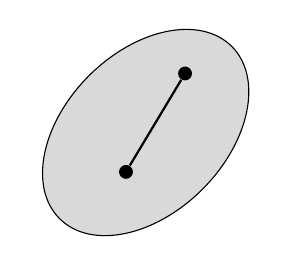
\begin{tikzpicture}
        \draw[rotate=-45,fill=gray!30] (0,0) ellipse (29pt and 44pt);
        \node[circle, fill=black,inner sep=0pt,minimum size=5pt] (A) at (0.5,0.75) {};
        \node[circle, fill=black,inner sep=0pt,minimum size=5pt] (B) at (-0.25,-0.5) {};
        \draw[thick] (A) -- (B) {};
        \end{tikzpicture}
        \caption{A convex set}
        \label{convex}
    \end{figure}
\end{frame}

\begin{frame}[t]{Formal Definitions}
    \begin{definition}[Convex Set]
        Given $k$ distinct points $p_1, p_2, \dots, p_k$ in $E^d$, the set of points
        \[p = \alpha_1 p_1 + \alpha_2 p_2 + \dots + \alpha_k p_k
        \; \; \; (\alpha_j \in \mathbb{R}, \alpha_j \geq 0, \alpha_1 + \alpha_2 + \dots \alpha_k = 1)\]
        is the \textit{convex set} generation by $p_1, p_2, \dots, p_k$, and $p$ is a \textit{convex combination} of $p_1, p_2, \dots, p_k$.   
    \end{definition}
    \begin{definition}
        Given an arbitrary subset of $L$ of points in $E^d$, the \emph{convex hull} conv(L) of $L$ is the smallest convex set containing $L$. 
    \end{definition}
\end{frame}

\begin{frame}{Mixing Things}
    \begin{itemize}
        \item Imagine you have the following 
        mixtures of substances:
    \end{itemize}
    
        \begin{table}[h]
            \centering
            \scalebox{0.8}{
            \begin{tabular}{c|c|c}
                subst. & fract. $A$ & fract. $B$\\ \hline
                $s_1$ & 10\% & 35\% \\  
                $s_2$ & 20\% & 5\% \\ 
                $s_3$ & 40\% & 55\% \\ \hline 
            \end{tabular}}
        \end{table}
    \begin{itemize}
        \item Using these substances can we create two other substances \\s $q_1$ and $q_2$?
    \end{itemize}
    \begin{table}[h]
            \centering
            \scalebox{0.8}{
            \begin{tabular}{c|c|c}
            \hline 
                $q_1$ & 25\% & 28\% \\  
                $q_2$ & 15\% & 15\% \\ \hline 
            \end{tabular}}
        \end{table}
\end{frame}

\begin{frame}[t]{Mixing Things}
\begin{itemize}
    \item Let's plot these values:
\end{itemize}
\begin{figure}
    \centering
\scalebox{0.6}{
    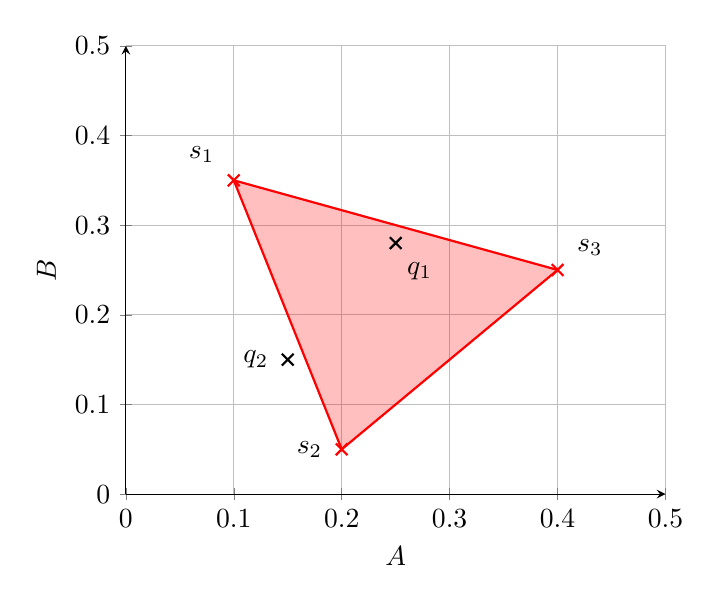
\begin{tikzpicture}
      \begin{axis}[
        grid=major,
          axis lines = left, 
          xlabel = $A$, 
          ylabel = $B$,
          xmin=0, xmax=0.5,
          ymin=0, ymax=0.5
          ]
          \addplot[
          fill=red,
          fill opacity=0.25,
          color=red,
          mark=x,
          mark size=3pt,
          thick
          ]
          coordinates{(0.1,0.35) (0.2, 0.05) (0.4, 0.25)};
          \addplot[
          color=red,
          mark=x
          mark size=4pt,
          thick
          ]
          coordinates{(0.1,0.35) (0.4, 0.25)};
          \addplot[
          color=black,
          mark=x,
          only marks, 
          mark size=3pt,
          thick
          ]
          coordinates{(0.25,0.28) (0.15,0.15)};
          \node[label={280:{$q_1$}}] at (axis cs:0.25,0.28) {};
          \node[label={180:{$q_2$}}] at (axis cs:0.15,0.15) {};
          \node[label={140:{$s_1$}}] at (axis cs:0.1,0.35) {};
          \node[label={180:{$s_2$}}] at (axis cs:0.2,0.05) {};
          \node[label={25:{$s_3$}}] at (axis cs:0.4,0.25) {};
      \end{axis}
    \end{tikzpicture}}
    \vspace{-1 em}
    \end{figure}
    \begin{itemize}
        \item We can observe that a substance $q \in \mathbb{R}^2$ can be created using 
        substances in $S \subset \mathbb{R}^2$ if and only if $q \in$ CH($S$).
    \end{itemize}
\end{frame}

\subsection{Problem Definition}
\begin{frame}{What is the Convex Hull Problem?}
    \begin{itemize}
        \item The convex hull problem is formally defined as:
        \begin{center}
        \begin{minipage}{0.75\textwidth}
          \begin{center}
            Given a set $S$ of $N$ points in $E^d$, construct its convex hull CH($S$).
          \end{center}
        \end{minipage}
      \end{center}
      \vspace{1 em}
      \item Another version of the convex hull problem is:
      \begin{center}
        \begin{minipage}{0.75\textwidth}
          \begin{center}
            Given a set $S$ of $N$ points in $E^d$, identify those that are vertices of conv($S$). 
          \end{center}
        \end{minipage}
      \end{center}
      \vspace{1 em}
      \item Both versions of the problem have the same asymptotic hardness since one problem can be 
      transformed to the other. 
    \end{itemize}    
\end{frame}

\begin{frame}[t]
  \frametitle{Convex Hull for Finite Set of Points}
    \begin{itemize}
      \item The convex hull for a finite set of points in the plane produces a convex polygon. 
    \end{itemize}
    \begin{figure}
      \centering
      \begin{subfigure}{0.35\textwidth}
        \centering
        \begin{tikzpicture}
          \node[circle, fill=black,inner sep=0pt,minimum size=2pt] (A) at (0,0) {};
          \node[circle, fill=black,inner sep=0pt,minimum size=2pt] (B) at (0,1) {};
          \node[circle, fill=black,inner sep=0pt,minimum size=2pt] (C) at (0.64,0.95) {};
          \node[circle, fill=black,inner sep=0pt,minimum size=2pt] (D) at (-0.6,0.7) {};
          \node[circle, fill=black,inner sep=0pt,minimum size=2pt] (E) at (-1,0.9) {};
          \node[circle, fill=black,inner sep=0pt,minimum size=2pt] (F) at (0.6,-0.5) {};
          \node[circle, fill=black,inner sep=0pt,minimum size=2pt] (G) at (-0.8,-0.4) {};
          \node[circle, fill=black,inner sep=0pt,minimum size=2pt] (H) at (-0.4,-0.1) {};
          \node[circle, fill=black,inner sep=0pt,minimum size=2pt] (I) at (0.25,0.5) {};
          \node[circle, fill=black,inner sep=0pt,minimum size=2pt] (J) at (-0.15,0.43) {};
          \node at (1, 1.25) {$P$};
        \end{tikzpicture}
      \end{subfigure}
      \begin{subfigure}{0.35\textwidth}
        \centering 
        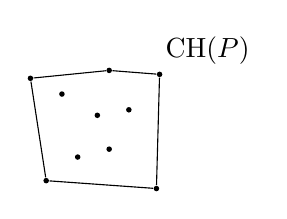
\begin{tikzpicture}
          \node[circle, fill=black,inner sep=0pt,minimum size=2pt] (A) at (0,0) {};
          \node[circle, fill=black,inner sep=0pt,minimum size=2pt] (B) at (0,1) {};
          \node[circle, fill=black,inner sep=0pt,minimum size=2pt] (C) at (0.64,0.95) {};
          \node[circle, fill=black,inner sep=0pt,minimum size=2pt] (D) at (-0.6,0.7) {};
          \node[circle, fill=black,inner sep=0pt,minimum size=2pt] (E) at (-1,0.9) {};
          \node[circle, fill=black,inner sep=0pt,minimum size=2pt] (F) at (0.6,-0.5) {};
          \node[circle, fill=black,inner sep=0pt,minimum size=2pt] (G) at (-0.8,-0.4) {};
          \node[circle, fill=black,inner sep=0pt,minimum size=2pt] (H) at (-0.4,-0.1) {};
          \node[circle, fill=black,inner sep=0pt,minimum size=2pt] (I) at (0.25,0.5) {};
          \node[circle, fill=black,inner sep=0pt,minimum size=2pt] (J) at (-0.15,0.43) {};
          \node at (1.25, 1.25) {CH($P$)};
          \shadedraw[] (B) -- (C) -- (F) -- (G) -- (E) -- (B);
        \end{tikzpicture}
      \end{subfigure}
      \caption{A point set and its convex hull.}
    \end{figure}
    \begin{itemize}
    \item In 3 dimensions however, the convex hull is not a convex polygon, but instead a 
    convex polyhedron -- generalizes to a polytope in higher dimensions.
  \end{itemize}
\end{frame}

\section{Convex Hull Algorithms \& Complexity}
\subsection{Lower Bound \& Output-Sensitivity}
    \begin{frame}[t]{Lower Bound on Computational Complexity}{Overview and Approach}
    \begin{itemize}
        \item The convex hull problem outputs a polygon -- a cyclic enumeration of the boundary vertices.
        \item We can say that we have to produce a sorting of the vertices.
        which has a lower bound of $\Omega(n\log n)$.
        \item To find lower bound of convex hull problem, we will reduce the sorting problem to the 
        convex hull problem in $O(n)$ time, which implies:
    \end{itemize}  
    \begin{theorem}
    Any algorithm for the convex hull problem requires $\Omega(n\log n)$ time in the worst case.
    \end{theorem}
    \end{frame}
    
    \begin{frame}[t]{Lower Bound on Computational Complexity}
    {Reduction of Sorting to Convex Hull}
\begin{itemize}
    \item Let $X = \{x_1, \dots, x_n\}$ be the $n$ values we wish to sort.
    \item We can "lift" each of these points onto a parabola $y=x^2$, by mapping $x_i$ to the point 
    $p_i=(x_i,x_i^2)$.
    \item $P$ is the resulting set of points -- all of which lie on the convex hull.
    \item The sorted order of points along the lower hull is the same as the sorted order $X$.
    \end{itemize}    
   \begin{figure}
       \centering
       \includegraphics[width=0.63\textwidth]{lowerbound.png}
       \vspace{-0.75 em}
       \caption{Reduction from sorting to convex hull.}
   \end{figure}
    \end{frame}

    \begin{frame}
      \frametitle{Output-Sensitive Algorithms}
      \begin{itemize}
          \item Some convex hull algorithms depend both on $n$ input points, 
          and $h$ output points. 
          \item Such algorithms are called \textit{output-sensitive} algorithms.
          \item They may be asymptotically more efficient than $\Theta(n\log n)$ algorithms when $h = o(n)$.
          \item The lower bound for these algorithms is $\Omega(n \log h)$ in the planar case. 
          \item Kirkpatrick and Seidel devised an algorithm that achieved this in 1986.
          \item In 1996, a much simpler algorithm was devised by Chan called Chan's algorithm.
      \end{itemize}
    \end{frame}

    \subsection{Algorithms}
    \begin{frame}{The General Position Assumption}
        \begin{itemize}
            \item Before we look at algorithms, let's look at an important 
            assumption. 
            \item We assume that the points are in \emph{general position}.
            \item This means that degenerate configurations do not arise in input. 
            \item Point sets in general position maintain general position if perturbed infinitesimally.
            \item Merely a convenience to avoid dealing with a lot of special cases during algorithm design.
        \end{itemize}
    \end{frame}

    \begin{frame}
      \frametitle[t]{Convex Hull Algorithms}
      \begin{itemize}
        \item There are multiple algorithms that employ different techniques to compute 
        the convex hull of a point set. 
        \item Following are some of these algorithms with their time complexity:
      \end{itemize}
        \begin{table}[h!]
            \centering
            \begin{tabular}{|c|c|}
                \hline 
                \textbf{Algorithm} & \textbf{Time Complexity}  \\ \hline 
                Jarvis March  & $O(nh)$ \\ \hline 
                Graham Scan & $O(n \log n)$ \\ \hline
                Quickhull & $O(n \log n)$ \\ \hline 
                Chan's Algorithm & $O(n \log h)$ \\ \hline 
            \end{tabular}
            \caption{Some algorithms and their complexities.}
            \label{tab:my_label}
        \end{table}
    \end{frame}
    
    \begin{frame}{Jarvis March}{Algorithm Description \& Visualization}
        \begin{itemize}
            \item Jarvis march a.k.a the gift wrapping algorithm, was published in 
            1973 by R. A. Jarvis.
            \item The algorithm begins with $i\leftarrow0$, and a point $p_0$ known to be on the convex hull. 
            \item Then it selects the point $p_{i+1}$ such that all points are to the right of the line segment $p_ip_{i+1}$.
            \item This can be done in $O(n)$ time by comparing polar angles.
            \item Let $i\leftarrow i+1$, and repeat until algorithm $p_h \leftarrow p_0$ again. 
            \item This would yield the convex hull in $h$ steps. 
            \item \href{https://upload.wikimedia.org/wikipedia/commons/9/9c/Animation_depicting_the_gift_wrapping_algorithm.gif}{\color{magenta}{Here is a link to an animation for Jarvis march.}}
        \end{itemize}
    \end{frame}
  
  
  \begin{frame}{Jarvis March}{Performance \& Time Complexity}
 \begin{columns}
\begin{column}{0.48\textwidth}
    \begin{itemize}
        \item Jarvis march is among the least efficient algorithms for 
        convex hull. 
        \item The algorithm loops $h$ times and within each iteration, it 
        loops $n$ times.
        \item Therefore, the time complexity is $O(nh)$.
    \end{itemize}
\end{column}
\begin{column}{0.46\textwidth}
    \begin{figure}
    \scalebox{0.75}{
    \centering
    \def\svgwidth{\columnwidth}
    \input{jarvisboy.pdf_tex}}
    \caption{The Jarvis march procedure.}
    \end{figure}
    \end{column}
    \end{columns}
  \end{frame}
  
 \begin{frame}[t]{Graham Scan}{Algorithm Description \& Visualization}
    \begin{itemize}
        \item Based on the \textit{incremental construction} technique.
        \item First, select the lowest point in the point set $P$ called point $p_0$.
        \item Sort all points cyclically w.r.t point $p_0$ based on polar angles.
        \item For each point, determine if travelling to that point constitutes a left turn or a right turn.
        \item If right turn: second-to-last point is not part of CH($P$) but lies inside.
        \item Do the same for previously visited points until 'left-turn set' is encountered.
        \item Repeat until starting point is reached in a counter-clockwise fashion. 
        \item \href{https://upload.wikimedia.org/wikipedia/commons/7/71/GrahamScanDemo.gif}
        {\color{magenta}{Link to visualization.}}
    \end{itemize}
 \end{frame}
  
\begin{frame}{Graham Scan}{Pseudocode}
\begin{center}
\scalebox{0.75}{
    \begin{algorithm}[H]
    \caption{GRAHAM SCAN}
    \KwIn{A point set $P$}
    \KwOut{The convex hull of $P$, CH($P$)}
    let $p_0$ be the minimum and left-most point in $P$ \\ 
    let $\langle p_1, p_2, \dots, p_n \rangle$ be the remaining points in $P$ sorted by polar angle in counterclockwise order around $p_0$ \\
    let $S$ be an empty stack \\
    PUSH($p_0, s)$ \\
    PUSH($p_1, S)$ \\
    PUSH ($p_2, S)$ \\ 
    \For{$i \leftarrow 3$ to $i \leftarrow n$}{
        \While{the angle formed by points TOP($S$) NEXT\_TO\_TOP($S$), and $p_i$ make a non-left turn}{
        POP($S$)
        }
        PUSH($p_i, S$)
    }
    \Return $S$
    \end{algorithm}
}
\end{center}
\end{frame}
 
\begin{frame}{Graham Scan}{Performance \& Time Complexity}
    \begin{itemize}
        \item Graham Scan is an efficient algorithm compared to Jarvis march.
        \vspace{0.25 em}
        \item The sorting procedure is done in $O(n \log n)$ time. 
        \vspace{0.25 em}
        \item The loop is $O(n)$ and not $O(n^2)$.
        \vspace{0.25 em}
        \item We visit each point at most twice -- once as a left turn and once as a right turn. 
        \vspace{0.25 em}
        \item The time to sort dominates the time complexity of the algorithm. 
        \vspace{0.25 em}
        \item Therefore, Graham scan is $O(n \log n)$.
    \end{itemize}
\end{frame}

\begin{frame}{Quickhull Algorithm}{The Philosophy Behind the Algorithm}
    \begin{itemize}
        \item The Quickhull algorithm is a divide-and-conquer algorithm. 
        \vspace{0.5 em}
        \item It is based on the strategy of triangular expansion. 
        \vspace{0.5 em}
        \item It is also used for computing convex hull in higher dimensions due to its efficiency. 
        \vspace{0.5 em}
        \item Quickhull also uses the prune-and-search approach, where the input size 
        is reduced by a constant factor at each step. 
        \vspace{0.5 em}
        \item Its working can be visualized \href{https://upload.wikimedia.org/wikipedia/commons/4/42/Animation_depicting_the_quickhull_algorithm.gif}{\color{magenta}{here}}.
    \end{itemize}
\end{frame} 

\begin{frame}[t]{Quickhull Algorithm}{Pseudocode for 2-Dimensional Quickhull}
\begin{enumerate}
    \item Find the points with minimum and maximum $x$-coordinates. 
    \item Use the line formed by the two points to divide the set into two subsets of points. 
    \item Determine the point, on one side of the line, with the maximum distance from the line --- forms a triangle with those of the line. 
    \item The points lying inside of that triangle cannot be part of the convex hull and can be ignored in later steps. 
    \item Repeat the previous two steps on the lines formed by the triangle (recursion). 
    \item Keep on doing so until no points are left. The points selected constitute the convex hull.
\end{enumerate}
\end{frame}

\begin{frame}{Quickhull Algorithm}{Visualization of Algorithm}
    \begin{figure}
    \begin{subfigure}{0.45\textwidth}
    \centering
    \scalebox{0.5}{
    \def\svgwidth{\columnwidth}
    \input{quickhull1.pdf_tex}}
    \caption{\footnotesize Steps 1 -- 2}
    \end{subfigure}
    \begin{subfigure}{0.45\textwidth}
    \centering
    \scalebox{0.5}{
    \def\svgwidth{\columnwidth}
    \input{quickhull2.pdf_tex}}
    \caption{\footnotesize Steps 3 -- 5}
    \end{subfigure}
    \vfill 
    \begin{subfigure}[b!]{0.45\textwidth}
    \centering
    \scalebox{0.5}{
    \def\svgwidth{\columnwidth}
    \input{quickhull3.pdf_tex}}
    \caption{Step 6}
    \end{subfigure}
    \end{figure}
\end{frame}

\begin{frame}{Quickhull Algorithm}{Performance \& Time Complexity}
    \begin{itemize}
        \item Finding the extreme points is an $O(n)$ operation.
        \item Quickhull divides into two sub-problems. 
        \item In the best case, the partition size is well-balanced:
        \[T(n) = 2 T(n/2) + O(n)\]
        \[T(n) = O(n \log n)\]
        \item Whereas, in the worst case this degenerates to $T(n) = n T(n-1) + cn$,
        which means the worst case is quadratic. 
    \end{itemize}
\end{frame}

\section{3D-Convex Hulls \& More}
\subsection*{Introduction}
\begin{frame}{The 3D Convex Hull Problem}
\begin{columns}[T]
\begin{column}{0.46\textwidth}
    \begin{itemize}
        \item Recall that in 3 dimensions, the convex hull is a polyhedron (3-polytope). 
        \item In this case, we are concerned with the \textit{facets} of a polytope.
        \item The convex polytope is the convex hull of all its vertices. 
        \item More complicated problem which is harder to visualize and implement. 
    \end{itemize}
\end{column}
\hfill
\begin{column}{0.4\textwidth}
    \begin{figure}
        \centering
        \includegraphics[width=0.8\textwidth]{3dhull.png}
        \caption{A 3-dimensional convex hull.}
    \end{figure}
\end{column}
\end{columns}
\end{frame}

\subsection*{Algorithms for 3D Convex Hulls}
\begin{frame}{The Gift-Wrapping Algorithm}
    \begin{itemize}
        \item The most famous and the simplest algorithm is the 
        gift wrapping algorithm. 
        \item 
    \end{itemize} 
\end{frame}

\begin{frame}{Other Approaches}
    
\end{frame}

\section*{References}
\begin{frame}{References}
          \begin{thebibliography}{10}
          
             \beamertemplatebookbibitems
          %   % Start with overview books.
          
             \bibitem{Author1990}
               A.~Author.
               \newblock {\em Handbook of Everything}.
    \newblock Some Press, 1990.

  \beamertemplatearticlebibitems
  % Followed by interesting articles. Keep the list short. 
  
  \bibitem{Someone2000}
    S.~Someone.
    \newblock On this and that.
    \newblock {\em Journal of This and That}, 2(1):50--100,
    2000.
  \end{thebibliography}
\end{frame}

\end{document}


